\documentclass[]{IEEEtran}
% some very useful LaTeX packages include:
%\usepackage{cite}      
\usepackage{graphicx}   
\usepackage{subfigure} 
\usepackage{url}       
\usepackage{amsmath}    
\usepackage{caption2}
% Your document starts here!
\begin{document}

% Define document title and author
	\title{Weekly Report}
	\author{Adviser: Prof. Yang Wen \\Student: Cheng Wensheng\\ Period: 2018.7.16-7.22
	}
	\markboth{Visual Information Processing Group}{}
	\maketitle

% Write abstract here
\begin{abstract}
	This week I mainly put my effort on testing the images given by contest committee and packing codes to EXE file.
\end{abstract}

% Each section begins with a \section{title} command
\section{Algorithm test}
	% \PARstart{}{} creates a tall first letter for this first paragraph
	\PARstart{S}{ince} contest committee gave some training SAR images, I used these images to train models. 
	\begin{itemize}
		\item The contest committee gave us 10 SAR building images, whose size is 1,500 $\times$ 1,500.  
		\item At first, I choose 7 images to train, 1 to validate and the last 2 to test. I slice theses images to small ones with size of 512 $\times$ 512 without overlapping. Finally I get 63 training images of 512 $\times$ 512.
		\item The result shows that the F1 score, which is used by the contest, is about 0.5 $\sim$ 0.6. This is on the average.
		
		Fig.~\ref{fig:mp} is the ground truth image. Fig.~\ref{fig:ss} is the predicted image.
	\end{itemize}

% Main Part
\section{Software packing}
	% LaTeX takes complete care of your document layout.
	According to the contest requirement, we need to pack codes to EXE format and run it on Win 7/10 with CUDA 8.0/9.0 platform.
	\begin{itemize}
		\item The code of SAR image building extraction uses TensorFlow framework. It supports Windows well and I run the code on Dell laptop with Win 10, CUDA 8 and Python 3.5 correctly.
		\item However, when I try to pack it with Pyinstaller, it reported some mistakes. After some trials, I changed the work directory in the code and it works as expected.
		\item Then I gave Lei Xu the code, and he mailed it to the appointed mailbox on Saturday.
	\end{itemize}
\newpage
\begin{figure}[!hbt]
%		 Center the figure.
		\vspace{0.3cm}
%		\hspace{50cm}
		\begin{center}
			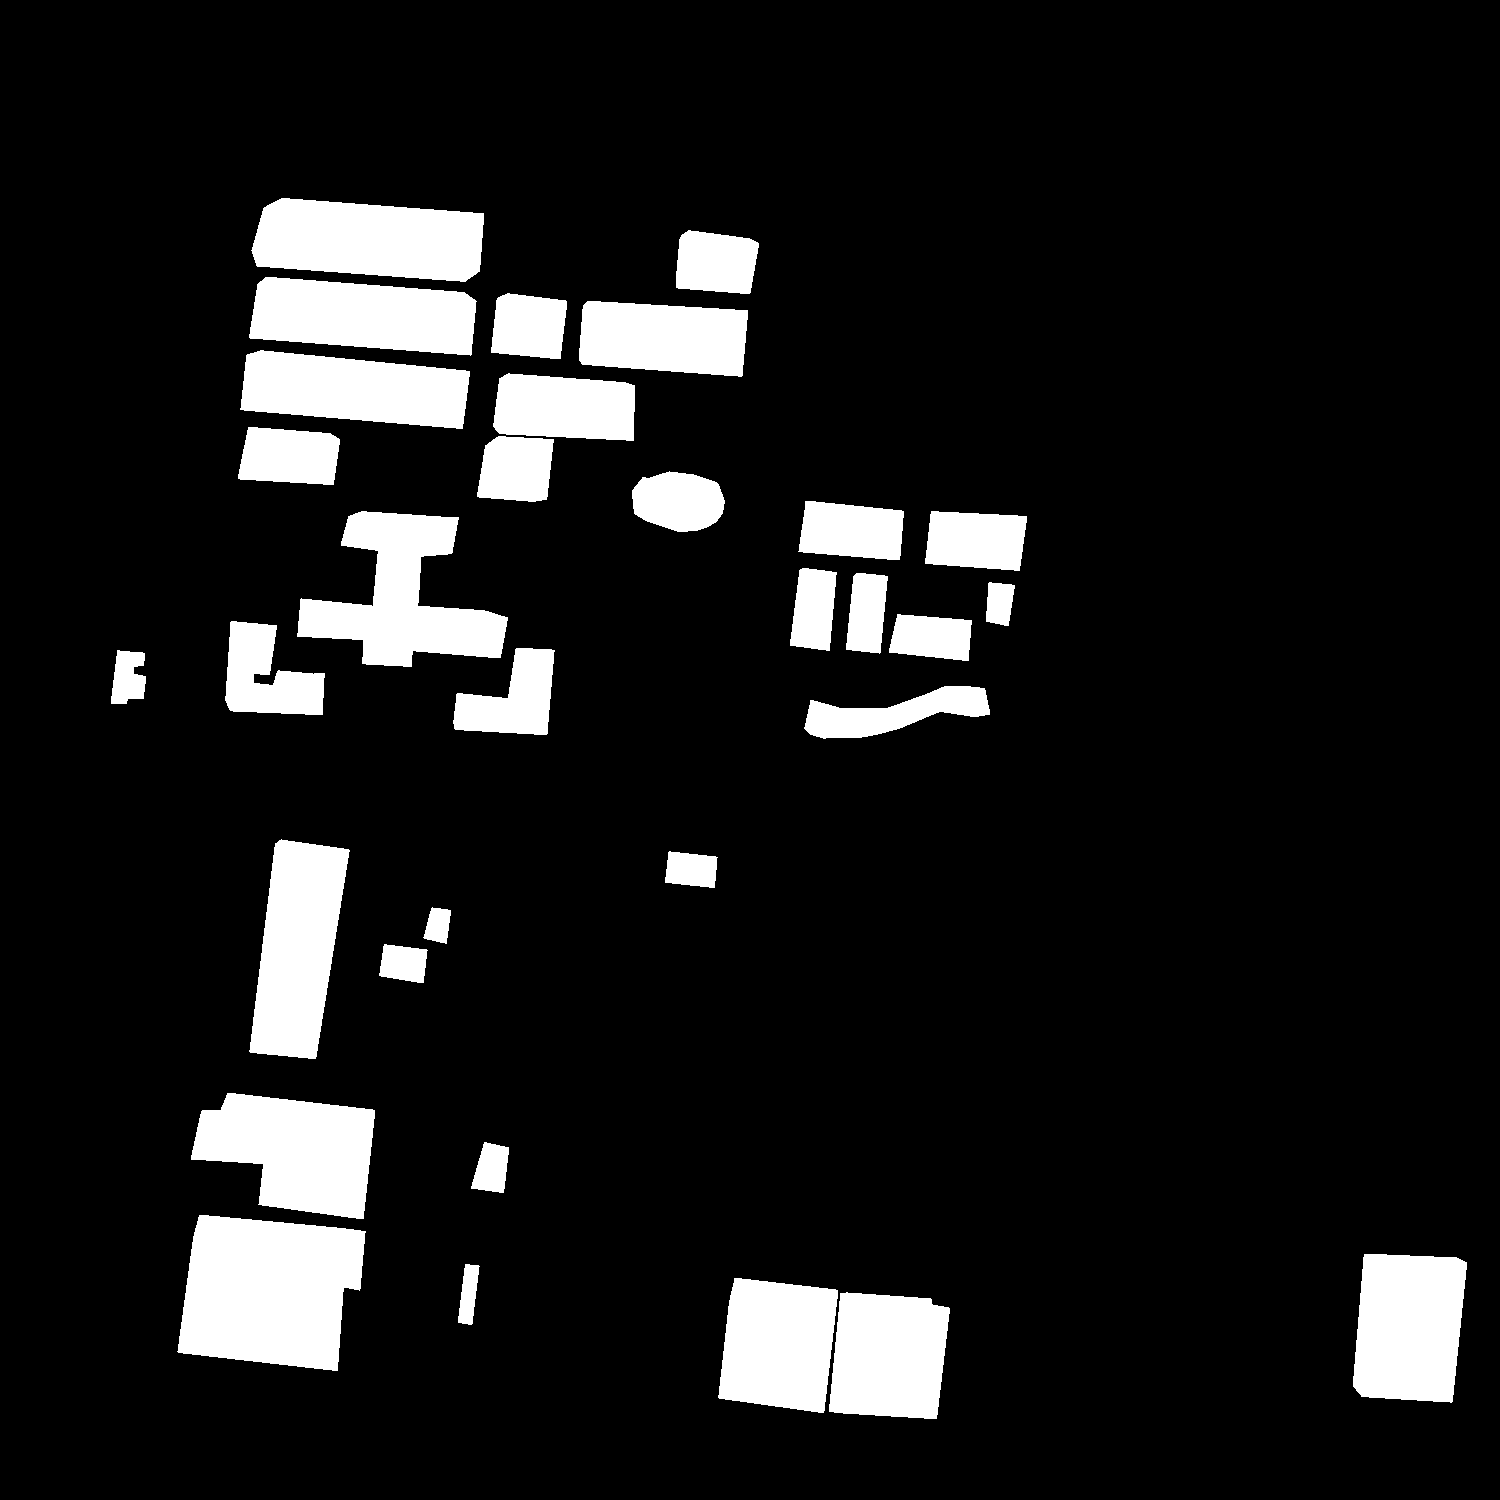
\includegraphics[width=0.7\columnwidth]{gt}
				%		 Create a subtitle for the figure.
			\caption{Ground truth image}
			\label{fig:mp}
		    \vspace{0.2cm}
			
\includegraphics[width=0.7\columnwidth]{pred}
				%Create a subtitle for the figure.
			\caption{Predicted image}
			\label{fig:ss}
		\end{center}
	\end{figure}

% Your document ends here!
\end{document}